% fig02_line.tex — standalone TikZ/pgfplots line example shipped with the template.
% Compiled by the paper Makefile via `make figures` (pdflatex on the snippet, no
% Python dep). Replace the `coordinates {...}` rows with your data; keep axis
% labels and the legend honest (units explicit, no log-scale without a label).
%
% IMPORTANT (working pattern): this is a STANDALONE document (own \documentclass).
% In main.tex, \includegraphics{figures/fig02_line.pdf} the COMPILED pdf — do NOT
% \input this .tex (that pulls a full \documentclass into your paper and breaks
% the build). `make figures` produces figures/fig02_line.pdf for you.
%
% Manual single-shot compile (debug):
%   pdflatex -interaction=nonstopmode -halt-on-error fig02_line.tex
\documentclass[tikz,border=4pt]{standalone}
\usepackage{pgfplots}
\pgfplotsset{compat=1.18}
\begin{document}
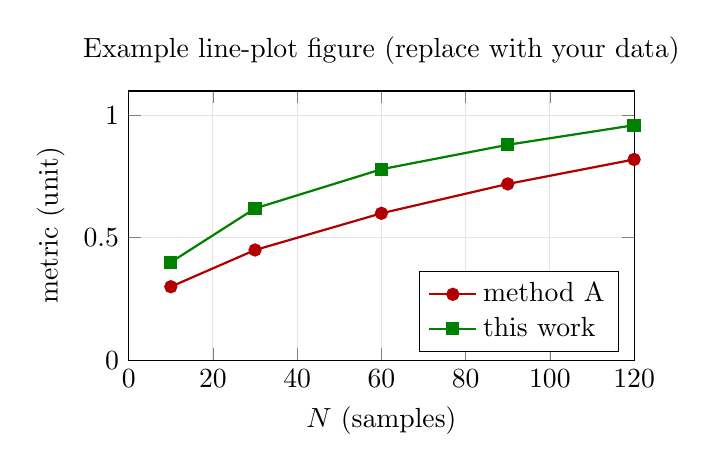
\begin{tikzpicture}
  \begin{axis}[
    width=8cm, height=5cm,
    xlabel={$N$ (samples)}, ylabel={metric (unit)},
    xmin=0, xmax=120,
    ymin=0, ymax=1.1,
    grid=both, grid style={gray!20},
    legend pos=south east, legend cell align=left,
    title={Example line-plot figure (replace with your data)},
  ]
    \addplot[mark=*, thick, color=red!70!black] coordinates {
      (10, 0.30) (30, 0.45) (60, 0.60) (90, 0.72) (120, 0.82)
    };
    \addlegendentry{method A}
    \addplot[mark=square*, thick, color=green!50!black] coordinates {
      (10, 0.40) (30, 0.62) (60, 0.78) (90, 0.88) (120, 0.96)
    };
    \addlegendentry{this work}
  \end{axis}
\end{tikzpicture}
\end{document}
